%% Le lingue utilizzate, che verranno passate come opzioni al pacchetto babel. Come sempre, l'ultima indicata sar� quella primaria.
%% Se si utilizzano una o pi� lingue diverse da "italian" o "english", leggere le istruzioni in fondo.
\def\thudbabelopt{english,italian}
%% Valori ammessi per target: bach (tesi triennale), mst (tesi magistrale), phd (tesi di dottorato).
%% Valori ammessi per aauheader: '' (vuoto -> nessun header Alpen Adria Univeristat), aics (Department of Artificial Intelligence and Cybersecurity), informatics (Department of Informatics Systems). Il nome del dipartimento � allineato con la versione inglese del logo UniUD.
\documentclass[target=bach,aauheader=]{thud}

%% --- Informazioni sulla tesi ---
%% Per tutti i tipi di tesi
% Scommentare quello di interesse, o mettete quello che vi pare
\course{Informatica}
%\course{Internet of Things, Big Data e Web}
%\course{Matematica}
%\course{Comunicazione Multimediale e Tecnologie dell'Informazione}
\title{Interfacce utente per la selezione \\ di item nel contesto di video giochi \\ in realtà virtuale immersiva}
\author{Paolo Casagrande}
\supervisor{Dott.\ Fabio Buttussi}
%\cosupervisor{Arch.\ Rambaldo Melandri \and Dott.\ Giorgio Perozzi}
%\tutor{Guido Necchi}
%% Campi obbligatori: \title, \author e \course.
%% Altri campi disponibili: \reviewer, \tutor, \chair, \date (anno accademico, calcolato in automatico), \rights
%% Con \supervisor, \cosupervisor, \reviewer e \tutor si possono indicare pi� nomi separati da \and.
%% Per le sole tesi di dottorato:
%\phdnumber{313}
%\cycle{XXVIII}
%\contacts{Via della Sintassi Astratta, 0/1\\65536 Gigatera --- Italia\\+39 0123 456789\\\texttt{http://www.example.com}\\\texttt{inbox@example.com}}

%% --- Pacchetti consigliati ---
%% pdfx: per generare il PDF/A per l'archiviazione. Necessario solo per la versione finale
\usepackage[a-1b]{pdfx}
%% hyperref: Regola le impostazioni della creazione del PDF... pi� tante altre cose. Ricordarsi di usare l'opzione pdfa.
\usepackage[pdfa]{hyperref}
%% tocbibind: Inserisce nell'indice anche la lista delle figure, la bibliografia, ecc.

%% --- Stili di pagina disponibili (comando \pagestyle) ---
%% sfbig (predefinito): Apertura delle parti e dei capitoli col numero grande; titoli delle parti e dei capitoli e intestazioni di pagina in sans serif.
%% big: Come "sfbig", solo serif.
%% plain: Apertura delle parti e dei capitoli tradizionali di LaTeX; intestazioni di pagina come "big".

% package per le immagini
\usepackage{graphicx}
\graphicspath{ {./images/} }

% package citazioni url
\usepackage{url}

\begin{document}
\maketitle

%% Dedica (opzionale)
%\begin{dedication}
%	Al mio cane,\par per avermi ascoltato mentre ripassavo le lezioni.
%\end{dedication}

%% Ringraziamenti (opzionali)
\acknowledgements
Ringrazio prima di tutto la mia Famiglia, che mi sostiene sempre e che mi ha dato piena fiducia nella scelta del mio percorso universitario.
Ringrazio il Dott. Fabio Buttussi, mio relatore, per avermi consentito di svolgere l'attività di tirocinio nel Laboratorio di Interazione Uomo Macchina e per avermi dato la possibilità di lavorare in un ambito che mi appassiona molto.
Ringrazio Alessandro Forgiarini per la pazienza e l'enorme aiuto che mi ha dato nel corso del tirocinio.
Ringrazio infine i miei Amici, grazie ai quali questi tre anni sono volati anche troppo in fretta.   

%% Sommario (opzionale) -> da mettere
%\abstract
%Nunc ac dignissim ipsum, quis pulvinar elit. Mauris congue nec leo ornare lobortis. Nulla hendrerit pretium diam nec lobortis. Nullam aliquam laoreet nisl, sit amet facilisis lectus accumsan ut. Duis et elit hendrerit metus venenatis condimentum. Integer id eros molestie, interdum leo sit amet, aliquet metus. Integer fermentum tristique magna, vel luctus neque rhoncus vel. Ut hendrerit et quam et semper. Mauris egestas, odio sed aliquet luctus, magna orci euismod odio, vitae lacinia tellus tellus non lectus. Aliquam urna neque, porta et mattis aliquam, congue sit amet lorem. In ultrices augue sit amet ante vehicula, vitae rhoncus turpis auctor. Donec porta scelerisque eros, at mollis enim imperdiet ut. 

%% Indice
\tableofcontents

%% Lista delle tabelle (se presenti)
%\listoftables

%% Lista delle figure (se presenti)
\listoffigures

%% Corpo principale del documento
\mainmatter

%% Parte
%% La suddivisione in parti � opzionale; solitamente sono sufficienti i capitoli.
%\part{Parte}
%\nocite{*} %% rimuovere magari in seguito
%% Capitolo
\chapter{Introduzione} % Introduzione alla VR + Intro dispositivi + Intro capitoli
\label{intro}
La Realtà Virtuale (Virtual Reality, VR) è un'interfaccia avanzata uomo-computer che simula un ambiente realistico \cite{Zheng}.
All'interno di questo ambiente l'utente è libero di muoversi, esplorare ed interagire con qualsiasi cosa, alimentando la sensazione di sentirsi effettivamente presente all'interno di un mondo virtuale.
Al giorno d'oggi, la Realtà Virtuale può essere applicata a vari settori tra cui l'intrattenimento, l'educazione, medico e commerciale. \\

L'interazione tra uomo e ambiente virtuale avviene attraverso specifici dispositivi.
L'interfaccia avanzata più utilizzata nella Realtà Virtuale è il visore VR. 
Questo visore, denominato Head Mounted Dispaly, può essere indossato come un casco che mostra all'utente il mondo virtuale a 360°.
Il visore VR utilizzato per l'esperimento è il Visore VR HTC Vive Pro, visibile in Figura \ref{fig:vive_pro}.

\begin{figure}[h]
    \centering
    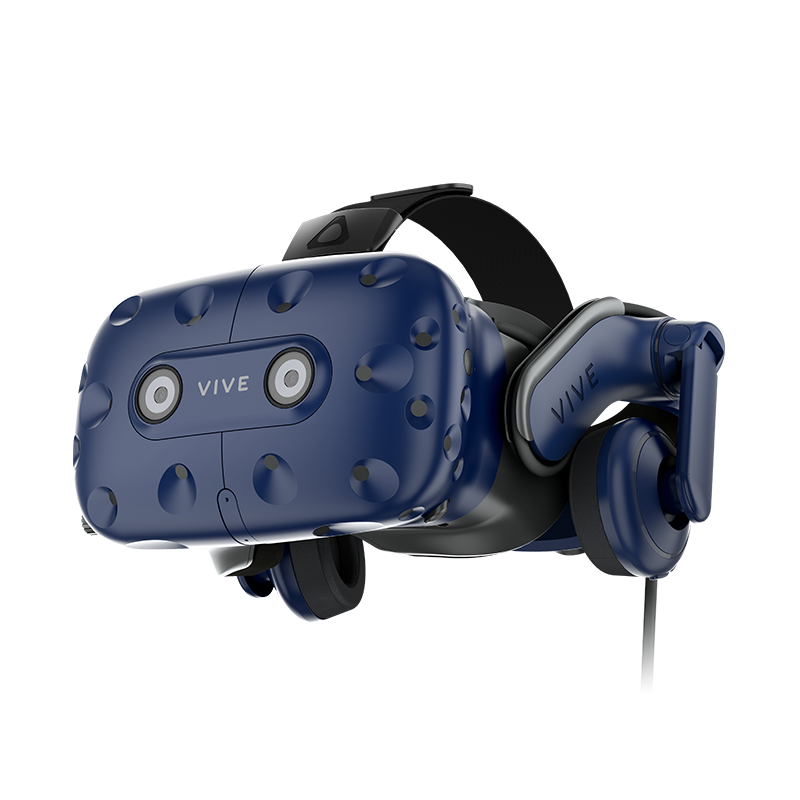
\includegraphics[width=0.25\textwidth]{vive_pro}
    \caption{Visore VR HTC Vive Pro}
    \label{fig:vive_pro}
\end{figure}

Insieme al visore, per interagire all'interno dell'ambiente virtuale, l'utente utilizza una coppia di controller per muovere entrambe le mani (Figura \ref{fig:vive_contr}).
Questi controller mappano il movimento delle mani nello spazio reale, che viene poi rappresentato nel mondo virtuale. 
L'utente può premere i tasti sui controller per esercitare azioni specifiche che interagiscono con l'ambiente virtuale. \\

\begin{figure}[h]
    \centering
    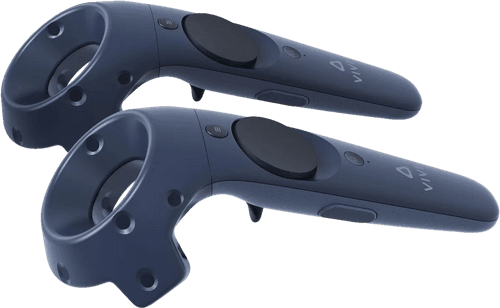
\includegraphics[width=0.25\textwidth]{vive_contr}
    \caption{Controller per HTC Vive Pro}
    \label{fig:vive_contr}
\end{figure}

\newpage
Quando si utilizza un visore VR le possibilità per gestire il movimento nell'ambiente virtuale sono:
\begin{itemize}
    \item Tramite joystick: ci si muove con l'aiuto di un controller;
    \item Leaning: bisogna inclinarsi verso la direzione nella quale si vuole andare;
    \item Walk in place: l'utente cammina sul posto nel mondo reale, muovendosi nello spazio virtuale;
    \item Teletrasporto: basta indicare con il controller una direzione verso la quale spostarsi virtualmente, rimanendo fermi nel mondo reale;
    \item Camminare nello spazio reale;
    \item Muoversi con una pedana per VR;
\end{itemize} 

Movimenti basati su joystick, leaning, teletrasporto o walk in place possono attenuare il senso di immersione nell'ambiente virtuale.
Per muoversi nel mondo reale, invece, bisogna avere a disposizione uno spazio ampio, altrimenti il rischio è di andare a sbattere da qualche parte senza vedere dove si va.
Una soluzione che permette di camminare nello spazio virtuale senza spostarsi realmente è la Pedana KAT WALK Mini S (Figura \ref{fig:kat_walk}).
Questa permette di spostarsi a 360° nel mondo virtuale, di correre, saltare e accovacciarsi. 
Bisogna indossare delle coperture sulla suola delle scarpe per creare l'effetto di pattinamento sulla pedana.    

\begin{figure}[h]
    \centering
    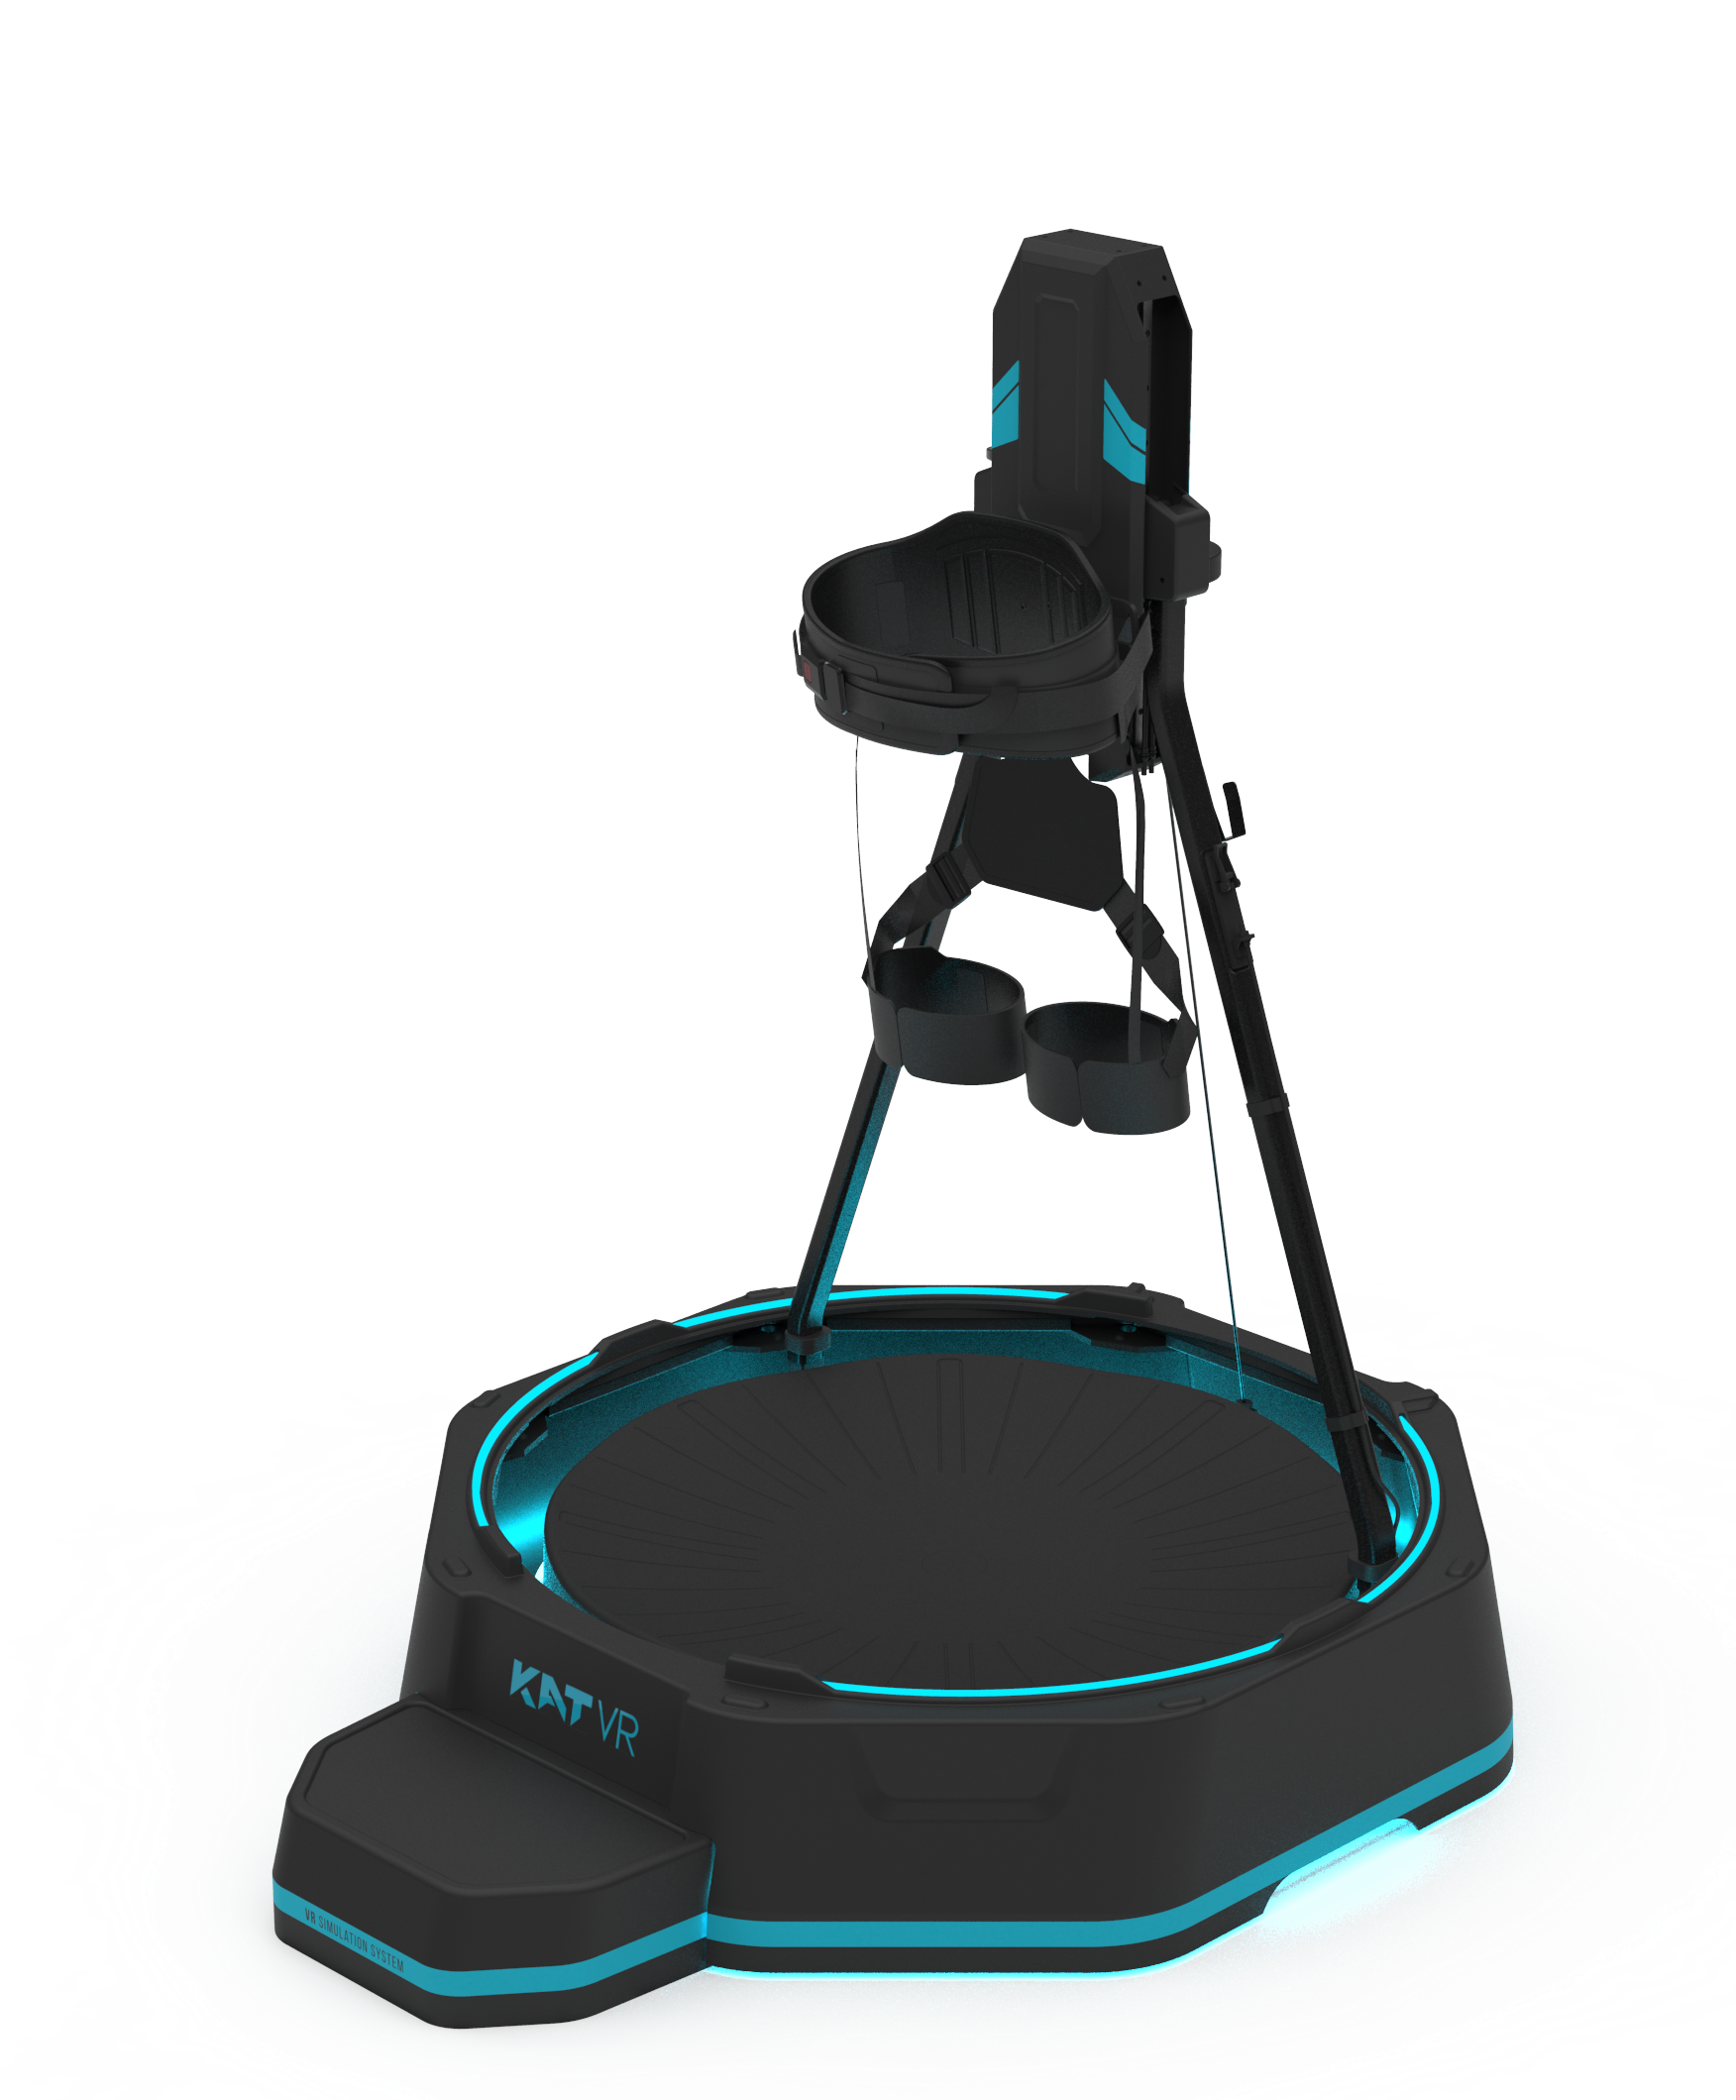
\includegraphics[width=0.40\textwidth]{kat_walk_mini}
    \caption{Pedana KAT WLK Mini S}
    \label{fig:kat_walk}
\end{figure}

L'obiettivo della tesi è quello di sviluppare un'interfaccia virtuale efficace che permetta agli utenti di selezionare determinati item.
L'efficacia dell'interfaccia dipenderà dalla facilità di selezione di un item, dalla rapidità con la quale lo si seleziona e dalla fatica che bisogna fare per selezionarlo.
Sono state progettate molte interfacce, come verrà spiegato meglio nei prossimi capitoli, per ottenere le due interfacce finali migliori. \\

L'utilizzo di questa interfaccia può essere generalizzabile ad altri oggetti che si potrebbe voler selezionare sia in giochi per l'intrattenimento sia in serious game.
Zyda \cite{Zyda} definisce i serious game come "una gara mentale, giocata con un computer secondo specifiche regole, che utilizza l'intrattenimento per favorire la formazione governativa o aziendale, l'istruzione, la salute, obiettivi di ordine pubblico e di comunicazione strategica".
Dunque i serious game sono giochi che si concentrano maggiormente sulla parte educativa rispetto a quella di intrattenimento.
Alcuni esempi di serious game sono stati approfonditi nel capitolo successivo \ref{art}. \\

Nel capitolo 2 viene descritto lo stato dell'arte riguardante la Realtà Virtuale e alcuni studi riguardo a interfacce in ambienti virtuali.
Nel capitolo 3 si spiega come sono state progettate tutte le interfacce, nel capitolo 4 le scelte di programmazione dell'ambiente virtuale.
Nel capitolo 5 si conclude la tesi parlando di ulteriori sviluppi futuri.

\chapter{Stato dell'arte} % Studi VR e interfacce + Legame tra VR e dispositivi
\label{art}
\section{VR immersiva e UI}
L'Interfaccia Utente (User Interface, UI) permette l'interazione tra uomo e macchina.
Fagerholt e Lorentzon \cite{Fagerholt} suddividono la rappresentazione dell'UI negli ambienti virtuali in 4 tipi di interfaccia:
\begin{itemize}
    \item Diegetica: l'UI è integrata all'interno dell'ambiente virtuale, ad esempio fondendosi con oggetti che ne fanno parte;
    \item Non-diegetica: l'UI viene mostrata fuori dal mondo virtuale, in sovrimpressione sullo schermo;
    \item Meta: sono interfacce 2D rappresentate nel mondo 3D che fanno parte del mondo virtuale;
    \item Spaziale: sono elementi UI 3D che non fanno parte del mondo virtuale e servono solo all'utente come informazione;
\end{itemize} 

Esistono molti studi che comparano diverse interfacce per interagire nelle applicazioni VR immersive.
Ad esempio, uno studio condotto da Hepperle et al. \cite{Hepperle} ha confrontato tre diverse interfacce - 2D, 3D e a comando vocale - per capire quale fosse la migliore per la Realtà Virtuale.  
Nello studio sono stati coinvolti 30 partecipanti, di cui 20 maschi e 10 femmine.
Degli utenti, solo il 66\% aveva esperienza con sistemi VR e il 50\% aveva già usato un dispositivo 3D prima d'ora.
La prova consisteva nel completare 17 compiti con le 3 interfacce nel minor tempo possibile e infine compilare un questionario.
I compiti comprendevano selezione, manipolazione, creazione, rotazione e modifica di oggetti virtuali.
Dai risultati è emerso che gli utenti, usando l'interfaccia sviluppata in 3D, consideravano l'input intuitivo e naturale; inoltre, rispetto alle altre interfacce, si sentivano più immersi nell'attività. \\

Uno studio di Raffaele et al. \cite{Raffaele} ha analizzato quale interfaccia immersiva fosse la migliore nei giochi VR.
Le interfacce a confronto proponevano rappresentazione spaziale, meta, diegetica e non-diegetica.
Allo studio hanno partecipato 50 utenti, che spaziavano tra designer, sviluppatori e videogiocatori.
I partecipanti dovevano infine compilare un questionario che paragonava 16 interfacce diverse utilizzate nei video giochi.
I risultati hanno mostrato che la rappresentazione diegetica è quella che permette la maggiore immersività di un'interfaccia in un ambiente virtuale. \\

Marre et al. \cite{Marre} hanno voluto testare quale interfaccia, tra non-diegetica e diegetica, fosse la migliore in un videogioco sparatutto.
Le informazioni sulla salute e munizioni dell'arma erano nel primo caso sovrapposti nello schermo, mentre nel secondo erano integrati nel mondo virtuale.
In questo studio sono stati coinvolti 41 partecipanti, composti da giocatori esperti e inesperti. 
Questa ricerca ha concluso che un'UI diegetica ha avuto un effetto positivo sulla performance degli utenti.
Questo studio conclude consigliando ai lettori di usare interfacce integrate il più possibile con il mondo virtuale. \\

Per quanto riguarda si serious game, ci sono stati molti studi per capire la relazione tra interfacce proposte e apprendimento degli utenti.
Infatti, uno studio di Rego et al. \cite{Rego} confronta diversi tipi di interfacce applicate in serious game riguardanti il campo della riabilitazione.
Dallo studio è emerso che le modalità di interazioni più naturali migliorano l'attrazione e l'intuitività di un serious game.

Feng et al. \cite{Feng} hanno sviluppato un serious game per insegnare come evacuare un ambiente tramite la Realtà Virtuale Immersiva.
Nel serious game sono state incluse emergenze come terremoti e incendi. 
Tramite questa applicazione gli utenti possono essere addestrati in particolari situazioni di emergenza in completa sicurezza.
Inoltre, al termine dell'esperienza possono essere annotati cambiamenti psicologici e fisici (battito cardiaco o fatica) degli utenti. \\

La tesi dunque si concentra dunque sullo sviluppo di interfacce per la selezione di item, partendo da soluzioni semplici e procedendo verso soluzioni sempre più immersive. 

\chapter{Design delle interfacce} % Percorso per arrivare alle interfacce adatte
\label{design}

Per sviluppare le interfacce è stata presa principalmente ispirazione dai video giochi, ma proseguendo con la progettazione sono stati raggiunti risultati originali. 
L'interfaccia deve permettere all'utente di selezionare degli item in maniera semplice e fluida, nel minor tempo possibile.
L'interfaccia deve anche essere utilizzabile mentre si cammina o si corre sulla pedana (Figura \ref{fig:kat_walk}) e non deve obbligare l'utente a fermarsi.
L'item che l'utente dovrà selezionare tramite l'interfaccia è una Chiave.
Ogni Chiave è caratterizzata da un colore diverso; questa scelta è trattata nella Sezione \ref{keys}.
L'ambiente di sviluppo per testare le interfacce è spiegato approfonditamente nella Sezione \ref{level}. \\

Per mostrare l'interfaccia bisogna premere il tasto Trigger, che è stato scelto perché che risulta semplice da premere ed è di facile accessibilità.  
L'interfaccia non deve rimanere sempre aperta, ma deve chiudersi una volta selezionata la Chiave che si vuole impostare come attiva (Figura \ref{fig:key_red}).
La Chiave attiva appare nella stessa mano che ha aperto il menu e può essere usata nel livello per aprire la Porta corrispondente.
Questo capitolo tratta in ordine lo sviluppo di tutte le interfacce, partendo dalle prime fino a raggiungere le due finali che sono state integrate nel progetto.

\begin{figure}[h]
    \centering
    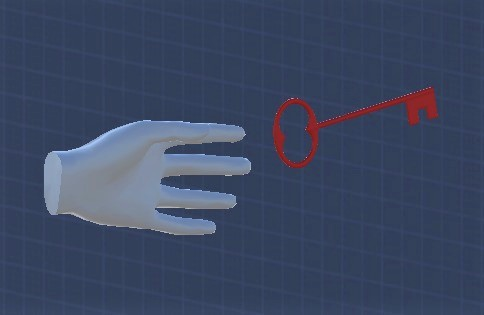
\includegraphics[width=0.60\textwidth]{key_red}
    \caption{Chiave Rossa impostata come attiva}
    \label{fig:key_red}
\end{figure}

I nomi di tutte le interfacce sono inventati e sono stati assegnati dal sottoscritto, Paolo Casagrande.

\section{Interfaccia Select} % < O >
\label{select}
L'interfaccia Select prende ispirazione dal menu di selezione rapido di \textit{Pokémon} del gioco \textit{Pokémon Legends Arceus}. 
Il menu si trova in basso a destra nella schermata (Figura \ref{fig:pok1}) e, come si vede meglio nel dettaglio (Figura \ref{fig:pok2}), è visibile in qualsiasi momento durante il gioco.
Questa interfaccia permette di permette cambiare il \textit{Pokémon} attivo in modo rapido in base alle esigenze. 
Nel gioco, si può usare il menu anche in movimento.

\begin{figure}[h]
    \centering
    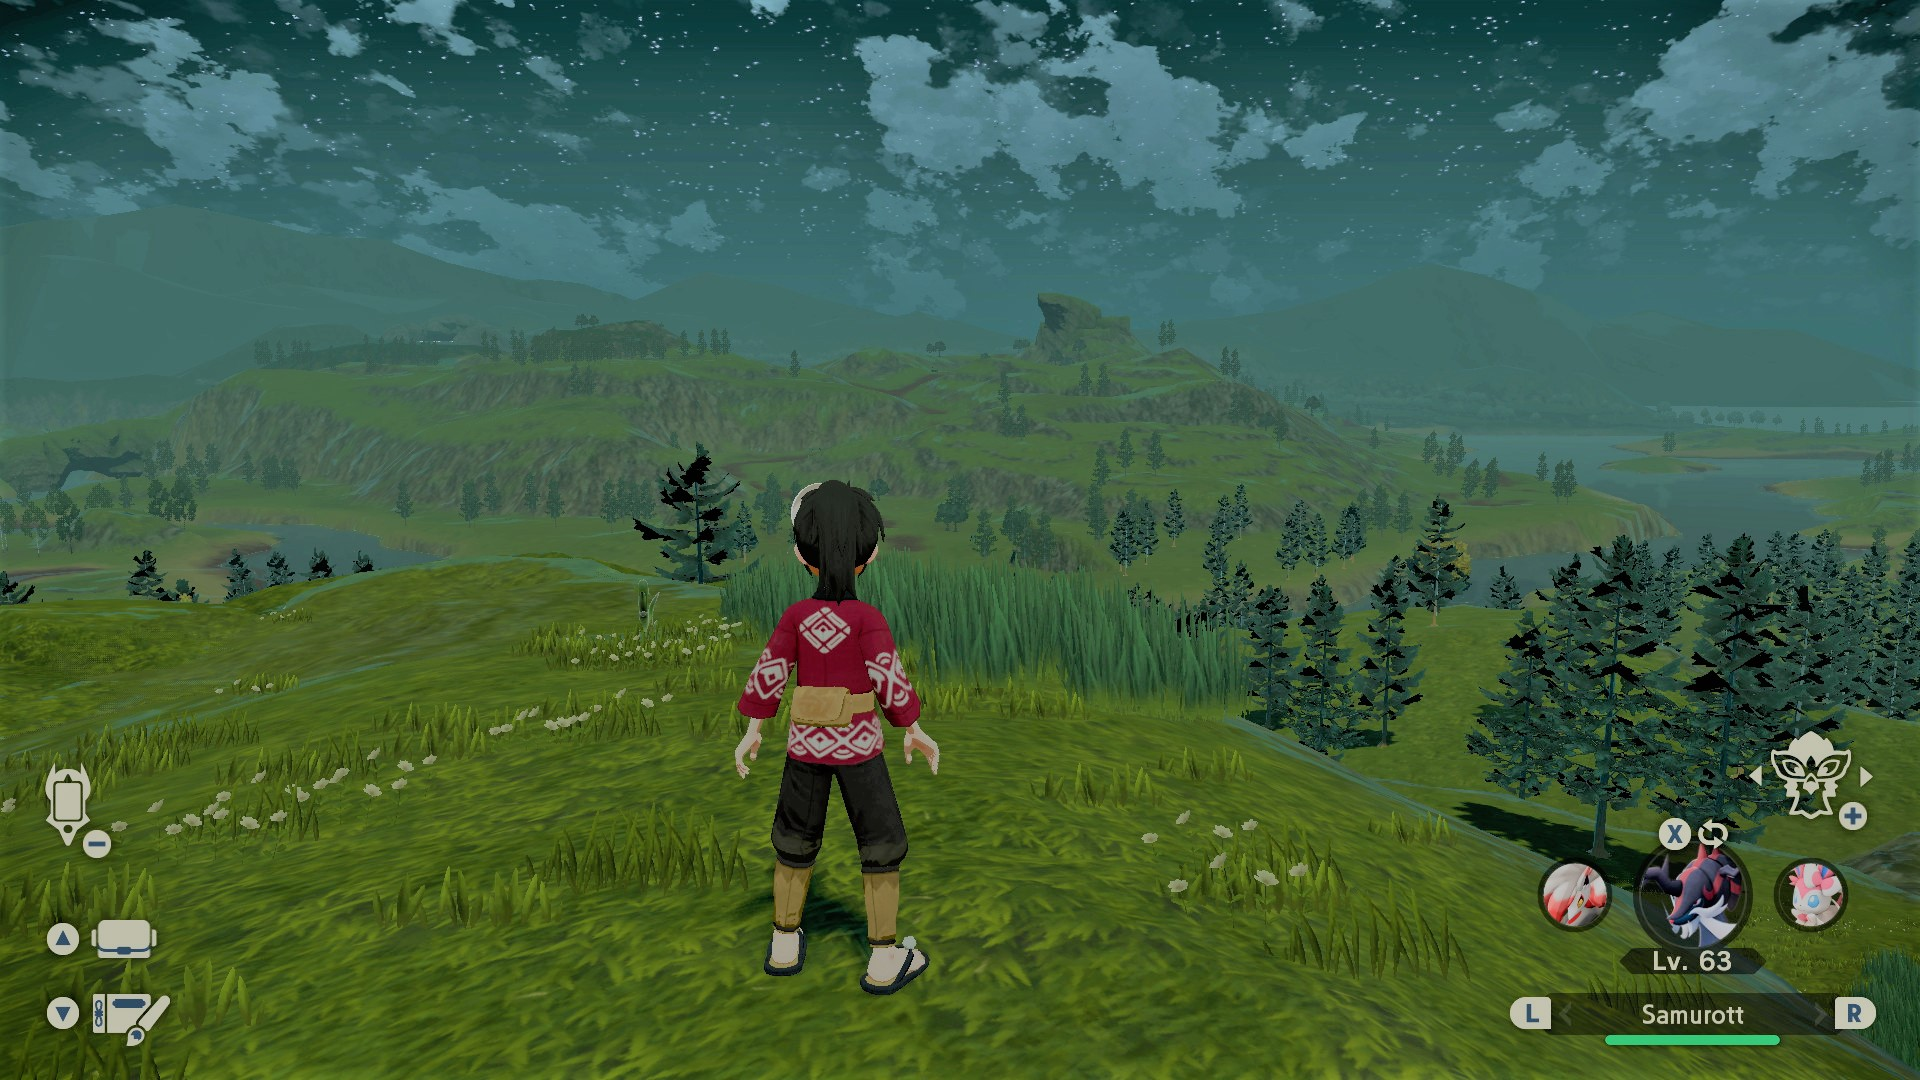
\includegraphics[width=0.60\textwidth]{pok1}
    \caption{Schermata di Pokémon Legends Arceus}
    \label{fig:pok1}
\end{figure}

\begin{figure}[h]
    \centering
    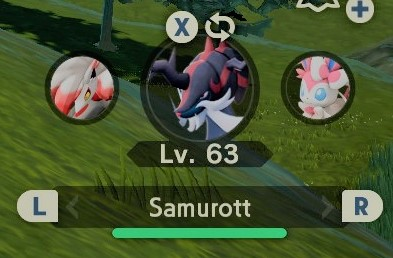
\includegraphics[width=0.60\textwidth]{pok2}
    \caption{Dettaglio dell'interfaccia di Pokémon Legends Arceus}
    \label{fig:pok2}
\end{figure}

Il concetto dell'interfaccia è stato semplificato in una Chiave 2D e due frecce disposte ai lati (Figura \ref{fig:select}).
Per aprire il menu bisogna tenere premuto il tasto Trigger.
Poi, premendo sulla freccia destra o sinistra del trackpad controller VR si può cambiare la Chiave attiva.
Rilasciando il Trigger il menu si chiude e lascia attiva la Chiave all'utente (Figura \ref{fig:key_red}).
Questo porta l'utente a premere due tasti con la stessa mano: uno va tenuto premuto e l'altro va cliccato quante volte si desidera. \\

Uno dei problemi di questa interfaccia è come vengono gestite le Chiavi.
All'inizio dello sviluppo sono stati utilizzati 8 colori assegnati ad ogni Chiave.
L'evoluzione dell'interfacce, come spiegato in seguito nella Sezione \ref{swish}, ha ridotto la scelta da 8 a 6.
A livello di codice, le Chiavi colorate vengono memorizzate in un vettore; premendo le frecce a destra o a sinistra si possono scorrere tutti gli elementi.
Bisogna notare che non c'è modo di saltare certi elementi, nè di vedere tra quanti elementi si otterrà quello desiderato.
Nel gioco di \textit{Pokémon Legends Arceus} questo tipo di menù viene usato sapendo bene l'ordine dei \textit{Pokémon} al suo interno.
L'utente, invece, non può conoscere in anticipo il contenuto del menu nè deve essere costretto a memorizzare l'ordine delle 8 Chiavi nel vettore.
Inoltre, tenere traccia di tutti gli item che scorre mentre cammina o corre può risultare difficile e macchinoso.
Sebbene quest'interfaccia risulti rapida da utilizzare, ci sono troppe limitazioni che la rendono poco utilizzabile nel contesto attuale.

\begin{figure}[h]
    \centering
    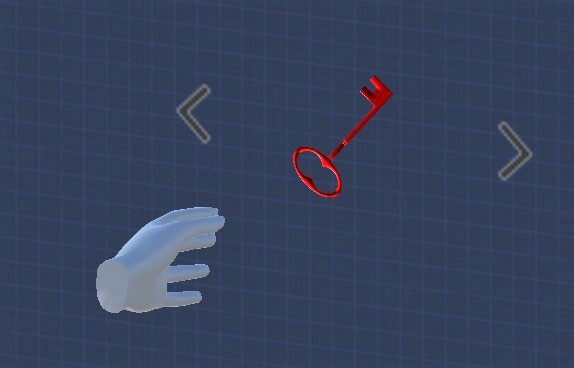
\includegraphics[width=0.60\textwidth]{select}
    \caption{Interfaccia Select}
    \label{fig:select}
\end{figure}


\section{Interfaccia Pie} % a torta
\label{pie}
L'interfaccia Pie si basa sul menu delle armi di \textit{Grand Theft Auto (GTA)}.
Il giocatore mette in pausa il gioco per selezionare un'arma da un menu a torta.
Una volta selezionata l'area dell'arma desiderata, il giocatore conferma la scelta premendo un pulsante.
Il gioco quindi esce dalla pausa e riprende.
Bisogna notare che questa suddivisione delle armi combacia con la scelta dei colori, ovvero 8. 
Qua sotto si può osservare un esempio dell'interfaccia trattata.

\begin{figure}[h]
    \centering
    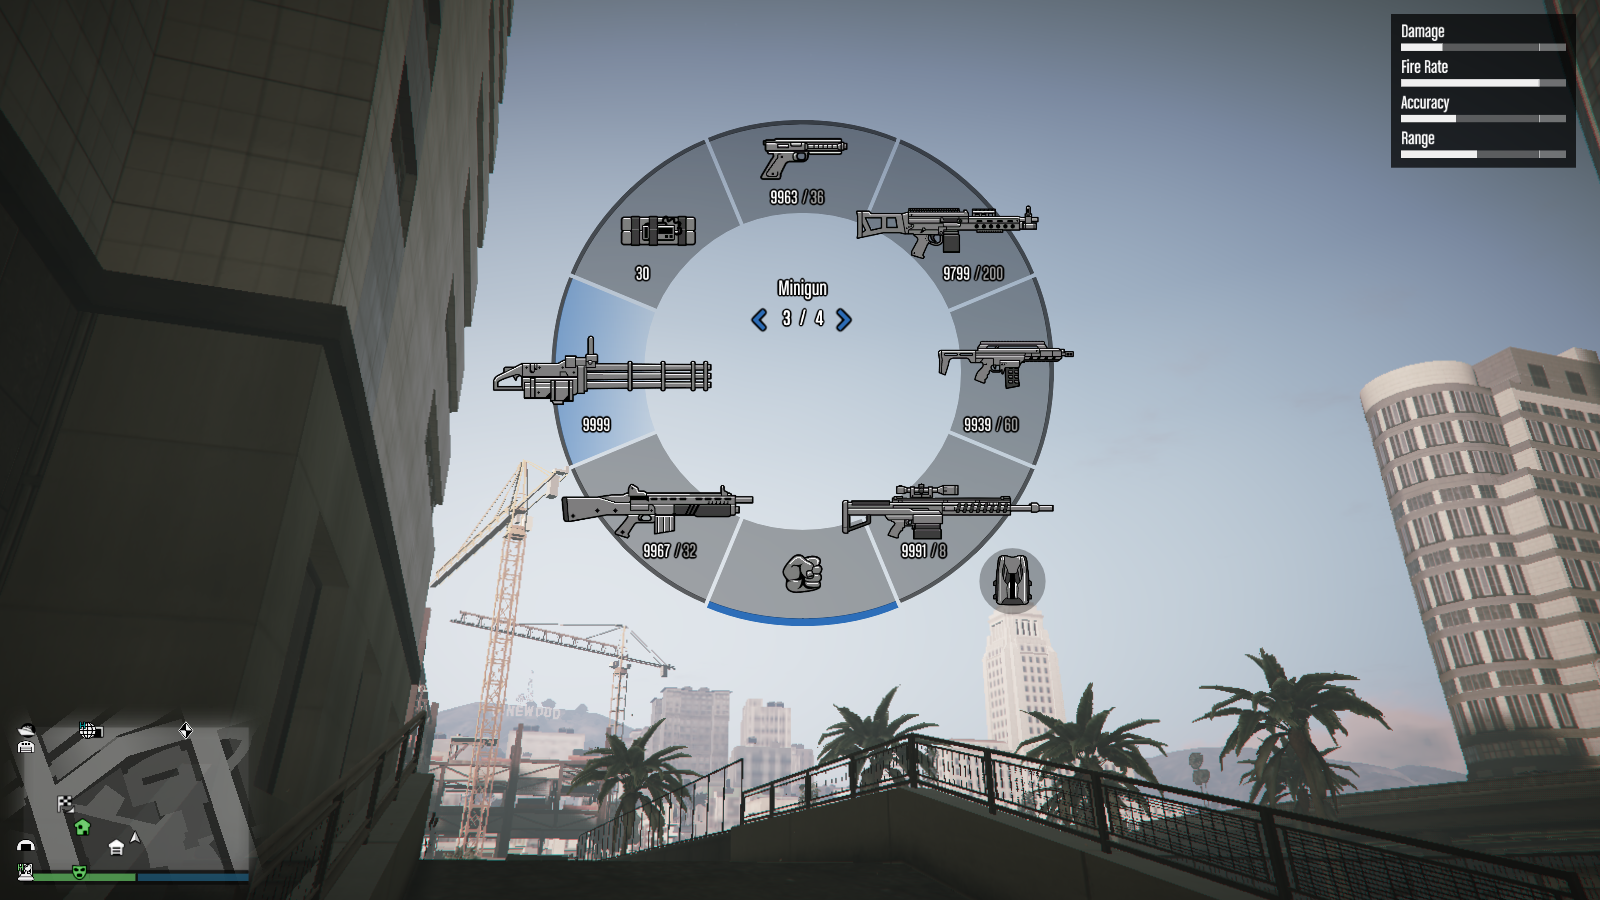
\includegraphics[width=0.60\textwidth]{gta}
    \caption{Interfaccia per la selezione di armi in GTA}
    \label{fig:gta}
\end{figure}

Altri esempi della stessa interfaccia sono presenti in molti video giochi, tra cui \textit{Assassin's Creed} e \textit{Animal Crossing: New Horizons}.

\begin{figure}[h]
    \centering
    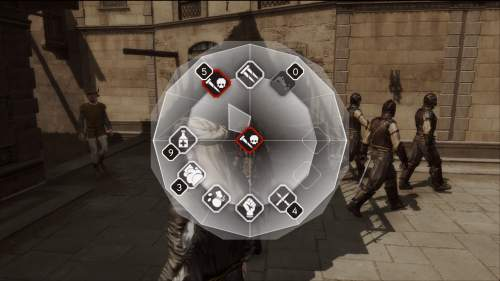
\includegraphics[width=0.40\textwidth]{ac}
    \caption{Interfaccia per la selezione di armi in Assassin's Creed}
    \label{fig:ac}
\end{figure}

\begin{figure}[h]
    \centering
    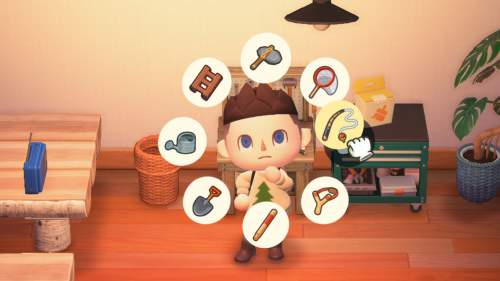
\includegraphics[width=0.40\textwidth]{nh}
    \caption{Interfaccia per la selezione di oggetti in Animal Crossing: New Horizons}
    \label{fig:nh}
\end{figure}

Ispirandosi a questo menu viene quindi sviluppata l'interfaccia Pie.
Scomponendo gli elementi principali del menu di \textit{GTA} si può notare che sono essenziali un cerchio per posizionare gli elementi e un'area per la loro selezione.
Ognuna delle 8 aree in cui è diviso il cerchio contiene uno dei colori delle Chiavi.
Anche in questo caso, il menu si apre tenendo premuto il tasto Trigger del controller.
Il cambiamento sta nel fatto che ora la selezione può avvenire a 360°.
Infatti, scorrendo con il pollice sul trackpad è possibile selezionare la Chiave del colore desiderato.
Infine, bisogna rilasciare il tasto Trigger per tenere in mano la Chiave scelta.
Nel cerchio tutti i settori sono grigi e per capire dove si trova un colore l'utente deve passarci sopra con il dito.

\begin{figure}[h]
    \centering
    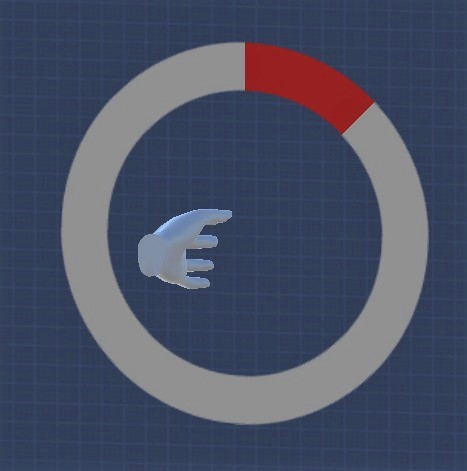
\includegraphics[width=0.45\textwidth]{pie}
    \caption{Interfaccia Pie}
    \label{fig:pie}
\end{figure}

L'interfaccia Pie presenta però dei problemi, alcuni molto simili all'interfaccia Select.
La selezione evidenzia soltanto un colore alla volta; l'utente non ha idea di dove si trovino gli altri colori e deve passarli tutti prima di avere un'idea chiara delle loro posizioni.  
Questo menu è ottimo se il gioco viene messo in pausa, mentre risulta complicato l'utilizzo quando si è in movimento.
Quando ci si muove, infatti, l'input risulta impreciso ed è molto facile commettere errori involontari nella selezione.
È necessario quindi trovare un movimento che non si basi solo su un dito, ma che coinvolga la mano o il braccio per catturare un input più intenzionale e consapevole.

\section{Interfaccia Swish} % bisogna indicare, scomodo
\label{swish}
L'interfaccia Swish, visibile in Figura (Figura \ref{fig:swish}), è l'evoluzione dell'interfaccia Pie nella Sezione\ref{pie}.

Quando viene premuto il tasto Trigger il menu si apre.
La particolarità di questo menu è che non serve premere altri pulsanti.
Infatti, per selezionare una Chiave bisogna indicare con il controller il colore desiderato e rilasciare il tasto Trigger.
Il codice prende in input il punto iniziale in cui è stato premuto il tasto Trigger e calcola la distanza e l'angolo dove viene rilasciato. \\

L'utente può vedere tutti i colori appena apre il menu, in modo da poter scegliere subito quale desidera.
In questo modo non perde tempo a cercare colori che venivano oscurati o nascosti dall'interfaccia.
Il movimento per la selezione della Chiave ricorda il movimento che braccio fa mentre si corre.

\begin{figure}[h]
    \centering
    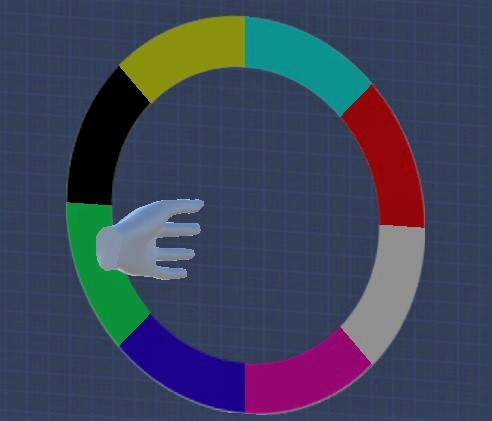
\includegraphics[width=0.50\textwidth]{swish}
    \caption{Interfaccia Swish}
    \label{fig:swish}
\end{figure}

Nello scorso paragrafo si è visto come l'interfaccia Swish prova a risolvere i problemi della precedente.
Ci sono però ancora delle questioni che lasciano libero spazio allo sviluppo.
Per prima cosa non è evidente quale colore si seleziona fino a quando non si ha la Chiave in mano.
Siccome il movimento è ampio e rapido, si rischia di sbagliare selezione.
Ciò comporta a dover aprire di nuovo l'interfaccia e ripetere la selezione. \\

Un altro problema che sorge riguarda il movimento del braccio durante la corsa.
Il movimento verso l'alto risulta naturale, ma i colori del cerchio posizionati in basso sono difficili da indicare per la selezione della Chiave.
Occorre quindi spostare in alto tutti i colori, in modo da semplificare il movimento e renderlo facilmente accessibile. 

\section{Interfaccia Lever}
\label{lever}
L'interfaccia Lever (Figura \ref{fig:lever}) presenta uno sviluppo significativo rispetto all'interfaccia Swish trattata nella Sezione \ref{swish}.
Per ridurre il numero di angoli da raggiungere con la mano si è passato da 8 a 6 colori. 
Sono stati quindi rimossi il colore bianco e nero ed il cerchio è stato considerevolmente ridotto di dimensioni.
L'apertura e selezione della Chiave viene effettuata come nel menu precedente.
Bisogna tenere premuto soltanto il tasto Trigger e rilasciarlo quando ci si trova nel colore che si vuole selezionare.
In questa interfaccia, però, il movimento della mano è cambiato. \\

Nel menù precedente, per indicare quale colore si volesse scegliere, la mano partiva da una posizione orizzontale e passava a verticale.
Questo effetto poteva ridurre la precisione del movimento, siccome la mano si spostava di parecchio durante la selezione.
Nell'interfaccia Lever la mano rimane sempre nella posizione verticale.
Il codice calcola l'angolo tra la mano in posizione verticale e l'asse orizzontale.
In questo modo si riesce a trovare la posizione precisa indicata dalla punta delle dita.
 
\begin{figure}[h]
    \centering
    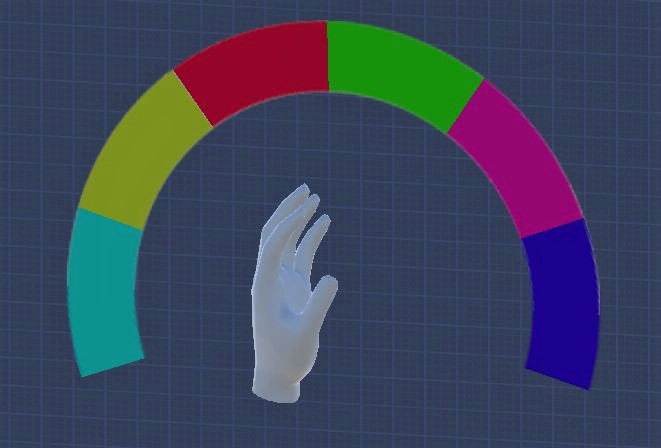
\includegraphics[width=0.60\textwidth]{lever}
    \caption{Interfaccia Lever}
    \label{fig:lever}
\end{figure}

L'innovazione di questa interfaccia è significativa e motstra molti miglioramenti rispetto alle precedenti.
Nonostante ciò, ci sono comunque degli aspetti negativi.
Durante la fase di movimento risulta scomodo tenere la mano in posizione perfettamente verticale.
Il movimento compiuto dalle braccia durante la corsa ostacola il funzionamento corretto dell'interfaccia.
Inoltre, nell'intervallo tra due settori del menu possono verificarsi imprecisioni durante la selezione.
Va notato inoltre notato che non viene ancora evidenziato in alcun modo il colore che l'utente vuole selezionare. 

\section{Interfaccia Wrist Rotation} % rotazione polso con lever menu 
\label{wrist_rot}
L'interfaccia Lever \ref{lever} viene migliorata con lo sviluppo dell'interfaccia Wrist Rotation (Figura \ref{fig:wrist_rot}).
L'unica cosa che cambia dall'interfaccia precedente riguarda il tipo di movimento che si esegue per selezionare una Chiave.
Prima la mano veniva tenuta in posizione verticale e andava inclinata in base a quale Chiave si volesse scegliere.
Con il nuovo tipo di movimento, attivare una determinata Chiave risulta più semplice.
Dal punto di vista del codice, bisogna pensare ad un asse immaginario che percorre polso, mano e controller.
L'angolo di rotazione attorno al polso viene calcolato e utilizzato per capire quale Chiave l'utente vuole selezionare.
L'apertura e chiusura è analoga alle interfacce precedenti, che funzionano tenendo premuto e rilasciando il pulsante Trigger. \\

Siccome il movimento per la selezione è l'unico cambiamento apportato, questa interfaccia presenta ancora tutti i lati negativi dell'interfaccia Lever trattata nella Sezione \ref{lever}.
Lo sviluppo dell'interfaccia Wrist Rotation, però, è un passaggio intermedio che si è dimostrato essere fondamentale per lo sviluppo di una delle due interfacce finali, di cui si parla nella Sezione \ref{int_wrist-spin}.

\begin{figure}[h]
    \centering
    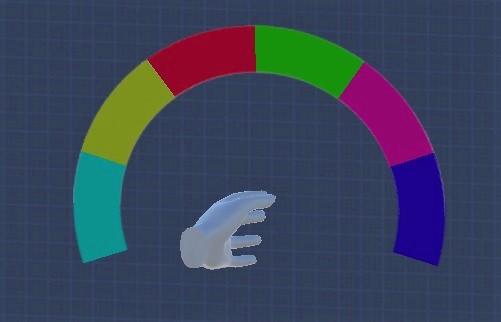
\includegraphics[width=0.60\textwidth]{wrist_rot}
    \caption{Interfaccia Wrist Rotation}
    \label{fig:wrist_rot}
\end{figure}

\section{Interfaccia Spin} % ruotare ad ogni chiave a destra o sinistra, evoluzione di select ma con rotazione polso
\label{spin}
Lo sviluppo dell' interfaccia Spin (Figura \ref{fig:spin}) si basa sul codice solido e semplice dell'interfaccia Select trattata nella Sezione \ref{select}; per questo il menu ha 8 colori.
La forma dell'interfaccia richiama quella di un anello portachiavi, ma è solo un altro modo di viualizzare il cerchio del menu Select.
Questa interfaccia è composta da un indicatore, che rimane fisso sulla posizione verticale; a ruotare sono tutte le Chiavi.
Il movimento su cui si basa la rotazione delle Chiavi è lo stesso del menu Wrist Rotation, affrontato nella Sezione \ref{wrist_rot}.
L'unica differenza è che per ogni pressione e rilascio del Trigger ci si può muovere a destra o a sinistra di una posizione. \\

\begin{figure}[h]
    \centering
    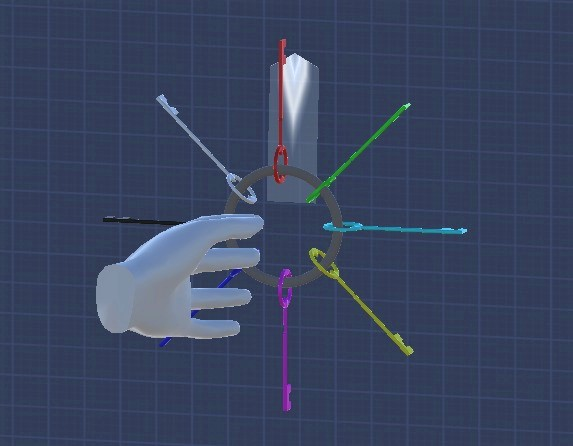
\includegraphics[width=0.60\textwidth]{spin}
    \caption{Interfaccia Spin}
    \label{fig:spin}
\end{figure}

L'interfaccia Spin presenta dei miglioramenti per l'immersività e per la chiarezza nella scelta della Chiave.
Però questo menu presenta molti problemi evidenti.
Ad esempio, ogni volta che viene rilasciato il Trigger viene selezionata una Chiave.
Dunque, se l'utente deve scegliere una Chiave opposta a quella precedentemente selezionata, dovrà attivare inutilmente molte Chiavi. 
Il movimento di rotazione del polso può risultare faticoso siccome viene ripetuto per un elevato numero di volte.
Inoltre, questa interfaccia è molto lenta e necessita di un'elevata attenzione per raggiungere la Chiave che si vuole scegliere.
Nato come una prova, il menu Spin ha mostrato vantaggi solidi ed è stato usato come base per creare una delle due interfacce finali \ref{int_wrist-spin}.  

\section{Interfaccia Finale 1: Wrist-Spin} % evoluzione wrist -> punti di forza di entrambi
\label{int_wrist-spin}
Lo sviluppo delle interfacce precedenti, soprattutto di Spin della Sezione \ref{spin} e Wrist Rotation della Sezione \ref{wrist_rot}, ha permesso la creazione di questa interfaccia.
Siccome è un ibrido tra Spin e Wrist Rotation, questa interfaccia è stata soprannominata Wrist-Spin e può essere vista nell'immagine sottostante (Figura \ref{fig:wrist_spin}).

\begin{figure}[h]
    \centering
    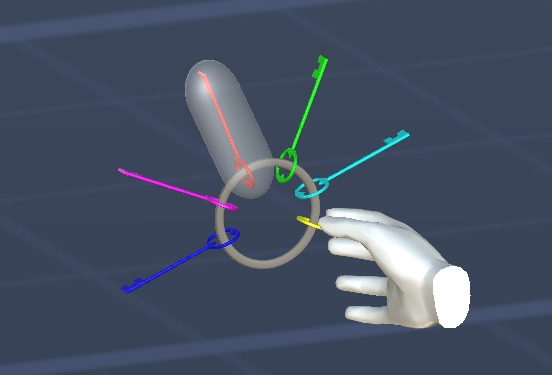
\includegraphics[width=0.60\textwidth]{wrist_spin}
    \caption{Interfaccia Wrist-Spin}
    \label{fig:wrist_spin}
\end{figure}

Questa interfaccia mostra numerosi aspetti positivi.
La pressione ed il rilascio del Trigger è rimasta inalterata dalle interfacce precedenti, risultando semplice ed efficace.
L'utente sa quale Chiave sta scegliendo perché questa viene evidenziata in modo evidente.
Il movimento dell'evidenziatore è settato con la posizione di ogni Chiave a livello di codice. 
Questo sigifica che non possono esserci situazioni intermedie o di incertezza, perché l'evidenziatore sarà sempre su una chiave.

I colori sono 6, così un utente non deve sforzarsi a piegare troppo il braccio in posizioni non usuali.
Questa interfaccia, durante lo sviluppo, non ha ostacolato i movimenti della corsa e sembra essere adatto per il tipo di attività che deve svolgere. 

\section{Interfaccia Finale 2: Spawn} % socket nelle mani a U
\label{int_spawn}
L'interfaccia Spawn (Figura \ref{fig:spawn}) è considerata finale perché è stata sviluppata dai vantaggi noti delle interfacce precedenti.
La differenza di questa interfaccia rispetto alle altre si può notare a livello di design.
Il tasto Trigger premuto su una mano fa apparire delle sfere colorate attorno all'altra mano dell'utente.
Tenendo premuto il Trigger, l'utente può toccare la sfera del colore che vuole scegliere.
Al rilascio del pulsante l'interfaccia si chiude e in mano rimane attiva la Chiave selezionata. 
Come riferimento si può osservare la Figura sottostante (Figura \ref{fig:spawn}). \\

\begin{figure}[h]
    \centering
    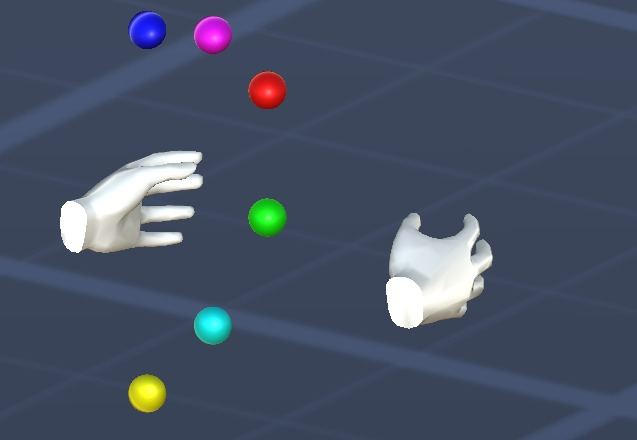
\includegraphics[width=0.60\textwidth]{spawn}
    \caption{Interfaccia Spawn}
    \label{fig:spawn}
\end{figure}

Questo menu utilizza la libreria Collider di Unity, trattando entrambe le mani dell'utente e tutte le sfere come Collider.
Il Collider è un'area attorno ad un oggetto, che può essere solida o attraversabile.
Il Collider è utile per identificare se ci sono collisioni tra oggetti diversi nell'ambiente virtuale.
In questa interfaccia i Collider servono per essere sicuri di selezionare un determinato colore.
Come si può notare dal particolare (Figura \ref{fig:coll}), i Collider sono molto piccoli e non c'è rischio da parte dell'utente di creare situazioni di imprecisione. \\

\begin{figure}[h]
    \centering
    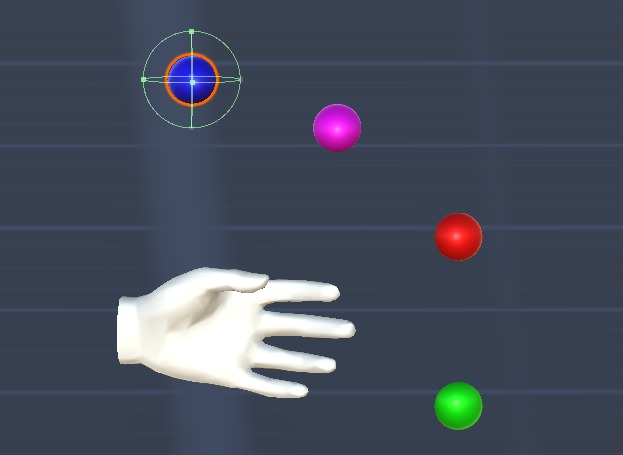
\includegraphics[width=0.60\textwidth]{coll}
    \caption{Particolare del Collider della sfera Blu}
    \label{fig:coll}
\end{figure}

\newpage 
Il movimento obbligatorio di questa interfaccia richiede che le mani si incrocino per selezionare una Chiave.
Questa azione avviene spontaneamente durante la corsa o la camminata, e non ostacola i movimenti.
Inoltre, la precisione della selezione è molto alta perché è l'utente stesso a muoversi come se fosse nella realtà.
Per questi motivi l' interfaccia non necessita di un evidenziatore per la selezione.
Inoltre, tutte le posizioni dei colori sono rese note appena l'utente apre il menu.
Così facendo può muoversi liberamente fin da subito senza che degli elementi risultino nascosti. 

\chapter{Progettazione dell'ambiente virtuale} % Spiegazione livello e menu vari + periferiche

In questo capitolo viene trattato lo sviluppo del livello, dei menu e di alcuni particolari dell'applicazione.

\section{Menu Iniziale}
\label{menu_init}
All'apertura dell'applicazione si presenta il Menu Iniziale (Figura \ref{fig:menu_screen}), dal quale si può scegliere una delle 4 voci:
\begin{itemize}
    \item Calibrazione Pedana: serve per calibrare la pedana in modo da spostarsi correttamente nell'ambiente virtuale;
    \item Test Pedana: fa provare la pedana attraverso un tutorial, spiegato in seguito nella Sezione \ref{tut_ped};
    \item Primo Menu e Secondo Menu: entrambe fanno provare un menu specifico, spiegato in seguito nella Sezione \ref{menu_int};
\end{itemize} 
Inoltre, l'intera attività può essere terminata premendo sulla "X" rossa in alto a destra.

\begin{figure}[h]
    \centering
    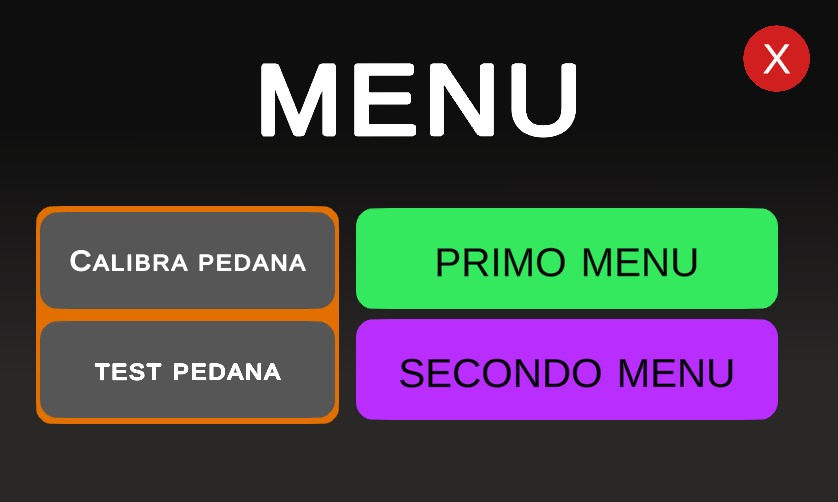
\includegraphics[width=0.60\textwidth]{menu_screen}
    \caption{Schermata del Menu Iniziale}
    \label{fig:menu_screen}
\end{figure}

\subsection{Sottomenu delle Interfacce}
\label{menu_int}
Dal Menu Iniziale si può scegliere quale delle due interfacce testare.
Questa schermata (Figura \ref{fig:first_menu}) presenta:
\begin{itemize}
    \item Tutorial: si può provare l'interfaccia senza fare il livello, spiegata in seguito nella Sezione \ref{tut_int};
    \item Gioca: si può accedere al livello, spiegato nel dettaglio alla Sezione \ref{level};
\end{itemize}
Inoltre è presente una freccia in alto a destra che permette di tornare alla schermata precedente, ovvero il Menu Iniziale trattato nella Sezione \ref{menu_init}.

\begin{figure}[h]
    \centering
    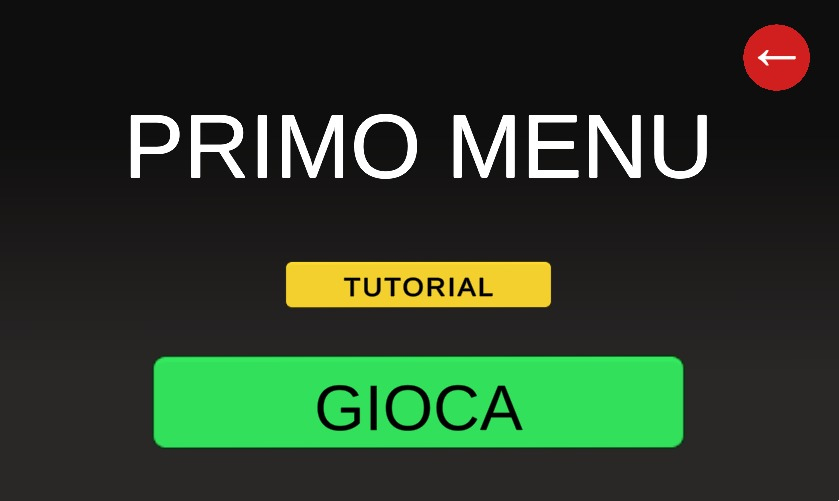
\includegraphics[width=0.60\textwidth]{first_menu}
    \caption{Schermata del Menu della Prima Interfaccia}
    \label{fig:first_menu}
\end{figure}

\section{Tutorial Design}
Pensando a questo progetto come una risorsa per eventuali test futuri su utenti, sono stati implementati due tipi di tutorial.

\subsection{Tutorial per la pedana}
\label{tut_ped}
Dal Menu Iniziale trattato nella Sezione \ref{menu_init} si può accedere a un tutorial per l'utilizzo della pedana.
Questo tutorial permette all'utente di muoversi in un ambiente chiuso e piatto.
L'utente può seguire dei tracciati tratteggiati posti sul terreno per acquisire familiarità con la pedana.
Inoltre nell'ambiente circostante sono stati posizionati degli oggetti 3D immobili e solidi per dare qualche punto di riferimento in più all'utente. 

\subsection{Tutorial per le interfacce}
\label{tut_int}
All'interno del Menu di ogni interfaccia, di cui si è parlato nella Sezione \ref{menu_int}, si può testare l'interfaccia scelta.
Le due interfacce sono i risultati dello sviluppo del progetto e all'interno del tutorial si può provarle con calma al fine di comprenderle al meglio.
Il tutorial presenta una struttura simile al livello ma senza la possibilità di cadere, cosa che verrà spiegata in seguito nella Sezione \ref{level}. 

\section{Level Design}
\label{level}
L'obiettivo della progettazione del livello consiste nell'obbligare l'utente ad interagire con l'interfaccia.
Si è pensato dunque di creare un corridoio dove il pavimento scompare con l'avanzare del tempo.
L'utente è quindi costretto a correre in avanti se vuole evitare di cadere e di perdere.
Lungo il corridoio sono state posizionate 6 porte che bloccano il passaggio, ognuna di un colore diverso.
L'utente deve selezionare una Chiave e toccare la Porta dello stesso colore per aprirla.
Ogni Porta che viene aperta aumenta di poco la velocità con cui il pavimento scompare. \\

L'utente supera il livello se riesce a raggiungere il traguardo posto alla fine del corridoio senza cadere.
Arrivando al traguardo, il pavimento viene bloccato e smette di scomparire.
In ogni istante, tramite un apposito script, viene controllata la posizione del giocatore.
Se l'utente cade deve ricominciare il livello.
L'intero percorso è visibile nell'immagine sottostante.

\begin{figure}[h]
    \centering
    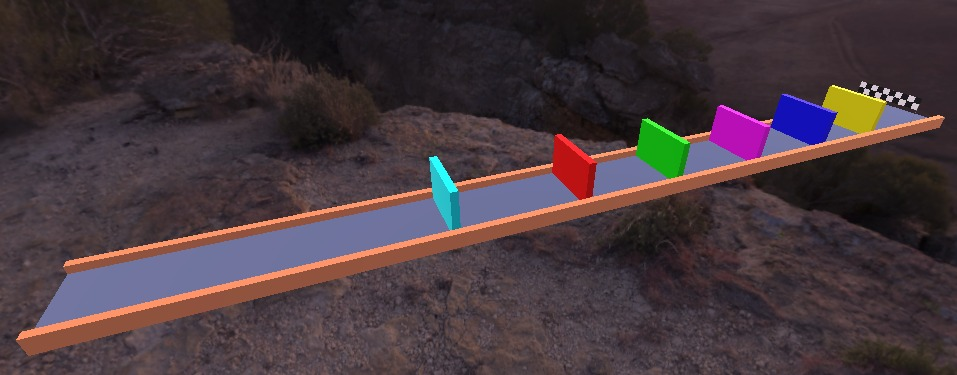
\includegraphics[width=0.60\textwidth]{level}
    \caption{Livello visto dall'alto}
    \label{fig:level}
\end{figure}

\section{Chiavi e Porte: scelta dei colori}
\label{keys}
Per distinguere sia le Chiavi che le porte si è pensato di assegnargli dei colori diversi.
I colori iniziali si basano sul modello HSB e comprendono 6 tonalità di colore diverse con l'aggiunta di bianco e nero (Figura \ref{fig:keys2}).

\begin{figure}[h]
    \centering
    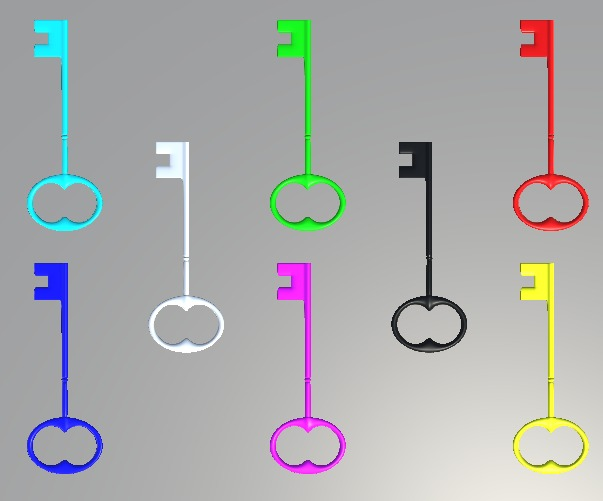
\includegraphics[width=0.50\textwidth]{keys2}
    \caption{Chiavi suddivise in 6 tonalità, con aggiunta di bianco e nero}
    \label{fig:keys2}
\end{figure}
%%%%%%%%%%%%%%
Durante lo sviluppo delle interfacce si è scelto di ridurre i colori a 6 tonalità, eliminando il bianco e il nero.
Solo in alcune interfacce iniziali i colori utilizzati sono stati 8: Select trattato nella Sezione \ref{select}, Pie trattato nella Sezione \ref{pie}, Swish trattato nella Sezione \ref{swish} e Spin trattato nella Sezione \ref{spin}. % ref ref
I motivi della riduzione delle tonalità da 8 a 6 sono affrontati nella Sezione \ref{swish}. % ref
I 6 colori scelti dunque sono rappresentati qua sotto (Figura \ref{fig:keys}). \\

\begin{figure}[h]
    \centering
    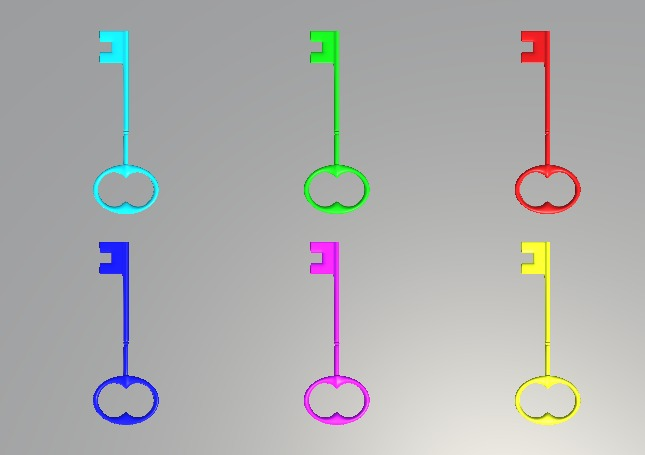
\includegraphics[width=0.60\textwidth]{keys}
    \caption{Chiavi suddivise in 6 tonalità}
    \label{fig:keys}
\end{figure}

Analogamente le porte collocate all'interno del livello possiedono gli stessi colori delle Chiavi.
Una Porta vista frontalmente appare come nella Figura sottostante (Figura \ref{fig:door}).

\begin{figure}[h]
    \centering
    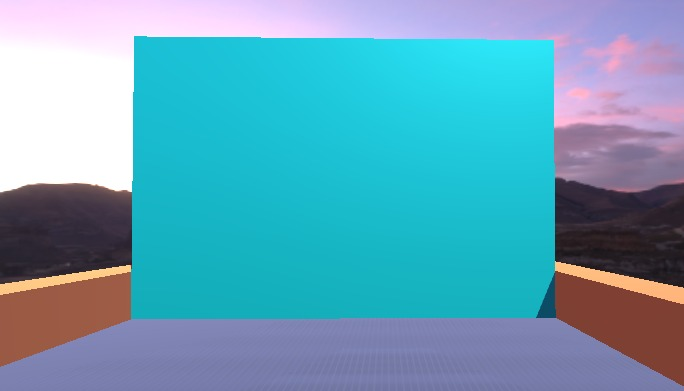
\includegraphics[width=0.60\textwidth]{door}
    \caption{Come viene vista la Porta Azzurra}
    \label{fig:door}
\end{figure}

\section{Funzionamento del livello}
L'utente può seguire le indicazioni sul Menu Iniziale della Sezione \ref{menu_init} e poi scegliere di affrontare un livello \ref{menu_int}.
Entrambi i livelli proposti sono uguali, presentando la stessa lunghezza del pavimento, stesso ordine delle porte e stessa velocità con la quale il pavimento scompare.
La differenza tra i due livelli riguarda quindi solo l'interfaccia utilizzabile per aprire le porte. \\

Cliccando quindi sulla voce Gioca dal Sottomenu delle Interfacce trattato nella Sezione \ref{menu_int}, l'utente carica il livello.
Si può notare qui sotto (Figura \ref{fig:lvl1}) la schermata visibile dall'utente appena inizia il livello.

\begin{figure}[h]
    \centering
    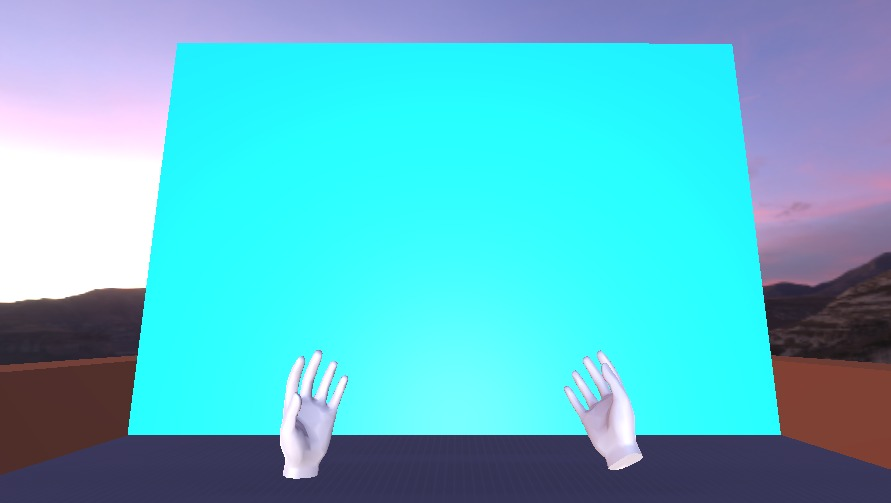
\includegraphics[width=0.50\textwidth]{lvl1}
    \caption{Punto di vista dell'utente all'inizio del livello}
    \label{fig:lvl1}
\end{figure}

\newpage
Segue poi l'apertura dell'interfaccia (Figura \ref{fig:lvl2}) per la selezione di una Chiave.
Tutti gli avvenimenti che riguardano le interfacce, le chiavi e le porte vengono memorizzati.
La raccolta dei dati è spiegata più approfonditamente nella Sezione successiva \ref{data}. \\

\begin{figure}[h]
    \centering
    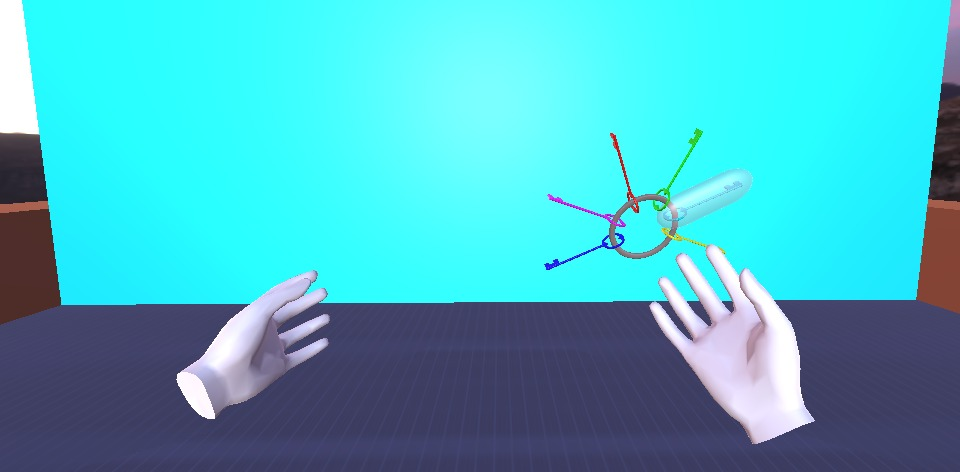
\includegraphics[width=0.50\textwidth]{lvl2}
    \caption{L'utente apre l'interfaccia per la selezione di una Chiave }
    \label{fig:lvl2}
\end{figure}

L'utente deve quindi avvicinarsi e toccare la Porta con la Chiave per aprirla (Figura \ref{fig:lvl3}).
Se la Chiave scelta è corretta, la Porta con cui l'utente ha interagito scompare (Figura \ref{fig:lvl4}). \\

\begin{figure}[h]
    \centering
    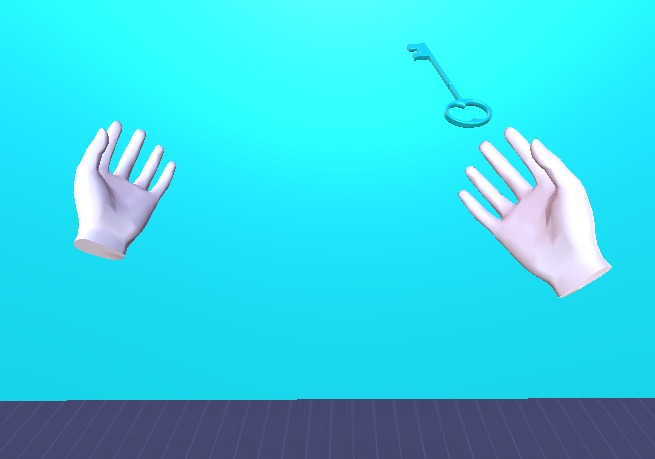
\includegraphics[width=0.50\textwidth]{lvl3}
    \caption{L'utente interagisce con la Porta Azzurra}
    \label{fig:lvl3}
\end{figure}

\begin{figure}[h]
    \centering
    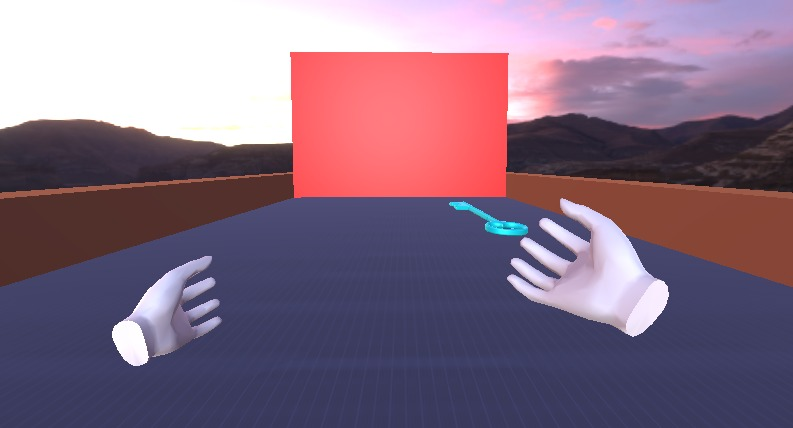
\includegraphics[width=0.50\textwidth]{lvl4}
    \caption{Apertura della Porta Azzurra}
    \label{fig:lvl4}
\end{figure}

\newpage
Una volta che sono state aperte tutte le Porte, l'utente deve raggiungere il traguardo posto alla fine del percorso (Figura \ref{fig:lvl5}).
Superato il traguardo, all'utente viene mostrata la schermata di completamento del livello (Figura \ref{fig:lvl6}). \\

\begin{figure}[h]
    \centering
    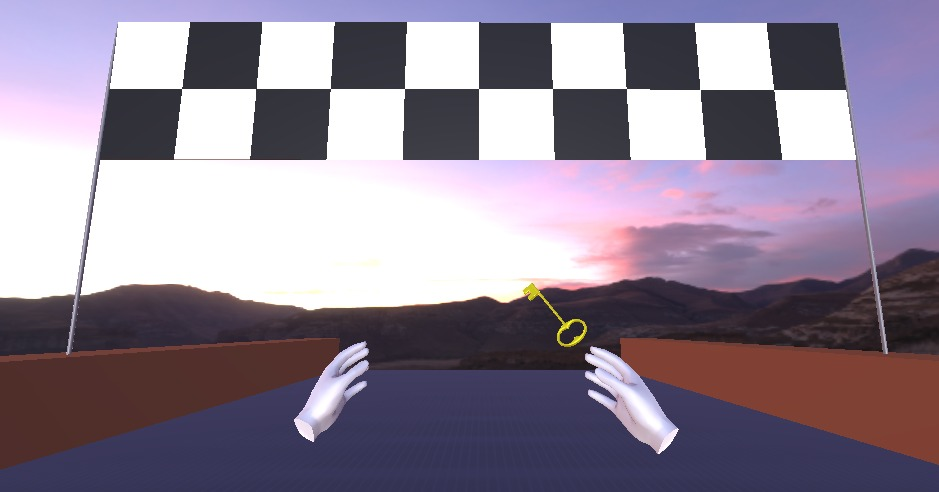
\includegraphics[width=0.60\textwidth]{lvl5}
    \caption{Raggiungimento del traguardo}
    \label{fig:lvl5}
\end{figure}

\begin{figure}[h]
    \centering
    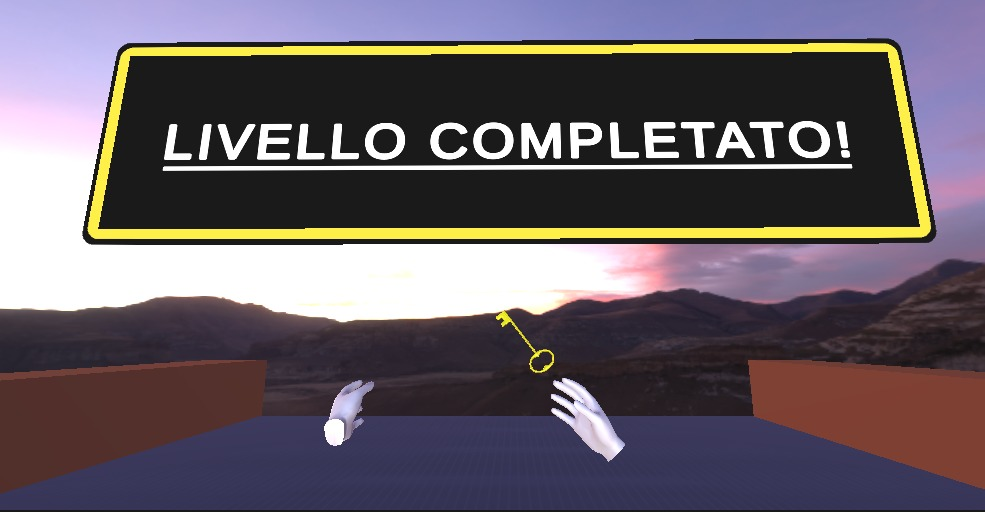
\includegraphics[width=0.60\textwidth]{lvl6}
    \caption{Completamento del livello}
    \label{fig:lvl6}
\end{figure}

Dopo aver terminato il livello, l'utente viene fatto tornare al Menu Iniziale nella Sezione \ref{menu_init}.
Tutti i dati raccolti vengono scritti tramite codice e registrtrati su appositi file JSON, come trattato nella Sezione seguente \ref{data}.

\section{Dati Raccolti}
\label{data}
Nell'applicazione è stata integrata una parte di acquisizione di dati, nel caso dovessero servire per fare dei test su utenti.
I file PlayerData.cs e PlayerInputFieldCode.cs permettono di raccogliere dati e scriverli ordinatamente su un file JSON.
Si può distinguere un giocatore da un altro inserendo un codice univoco all'apertura del programma (Figura \ref{fig:cod}).

\begin{figure}[h]
    \centering
    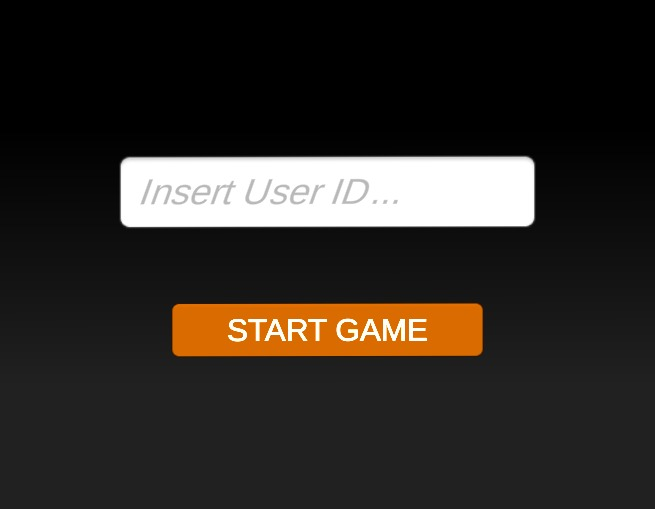
\includegraphics[width=0.60\textwidth]{cod}
    \caption{Campo per l'inserimento del codice univoco}
    \label{fig:cod}
\end{figure}

Così facedo, tutti i dati verranno salvati su un file chiamato come il codice di formato JSON.
I dati raccolti dagli utenti che provano l'applicazione sono i seguenti:
\begin{itemize}
    \item Numero totale delle morti nel primo livello;
    \item Numero totale delle morti nel secondo livello;
    \item Tempo di distruizone e collisioni con le Porte del primo livello;
    \item Tempo di distruzione e collisioni con le Porte del secondo livello;
    \item Chiavi selezionate e tempo totale del primo livello
    \item Chiavi selezionate e tempo totale del secondo livello;
\end{itemize}

Inoltre, ogni interfaccia finale può essere utilizzata sia dal controller della mano destra che dal controller della mano sinistra.
Questo perché in caso di necessità in eventuali test non vi siano problemi se un utente preferisce usare la mano destra o sinistra.

\section{Software Utilizzati}
Per programmare un ambiente virtuale interagibile tramite visore VR e pedana KAT WALK è stato utilizzato il game engine Unity.
Per potersi interfacciare con la pedana e calibrarla è stato usato il KATVR SDK, un plug-in sviluppato appositamente da KATVR.
Le icone delle Chiavi della Sezione \ref{keys} sono state generate usando il \href{https://github.com/AndreaDev3D/ThumbCreator}{plug-in di Unity “ThumbCreator” di AndreaDev3D}.
Infine, il plug-in OpenXR ha permesso di interfacciare l'ambiente in Unity con il visore HTC Vive Pro.


\chapter{Conclusioni} % cosa si può fare
Sviluppando le interfacce trattate nella tesi sono emersi molti fattori positivi che costituiscono un'interfaccia VR.
Le considerazioni per sviluppare una buona interfaccia per la Realtà Virtuale si possono così riassumere:
\begin{itemize}
    \item Mostrare ogni elemento dell'interfaccia, senza tenere nascosto nulla;
    \item Il movimento per selezionare l'item deve essere consono all'attività che l'utente deve svolgere;
    \item L'interfaccia deve fornire un indicatore che evidenzi in modo evidente quale item l'utente sta selezionando;
    \item L'interfaccia deve essere semplice da aprire e chiudere, senza essere troppo macchinosa o complicata;
    \item L'interfaccia deve mantenere una linea di coinvolgimento e di immersivita con l'ambiente virtuale che la circonda; \\
\end{itemize}

Un possibile sviluppo futuro potrebbe essere il test dell'applicazione e delle interfacce finali da parte di un gruppo di utenti.
Come accennato in precedenza nella Sezione \ref{data}, l'applicazione è già predisposta per la raccolta di dati da entrambe le interfacce.
I dati raccolti dall'applicazione, accompagnati da un questionario per ogni interfaccia testata, potrebbero comporre uno studio in grado di definire l'immersività o l'utilità di entrambe le interfacce. \\

L'obiettivo di sviluppare delle interfacce per la selezione di item nella la Realtà Virtuale è stato raggiunto.
I problemi e gli errori delle interfacce iniziali sono stati utili perché hanno portato ad un'implementazione sempre più mirata e efficace per il tipo di attività che la tesi ha richiesto.

%% Fine dei capitoli normali, inizio dei capitoli-appendice (opzionali)
%\appendix
%\part{Appendici}
%\chapter{Titolo della prima appendice}

%% Parte conclusiva del documento; tipicamente per riassunto, bibliografia e/o indice analitico.
\backmatter

%% Riassunto (opzionale)
%\summary
%Maecenas tempor elit sed arcu commodo, dapibus sagittis leo egestas. Praesent at ultrices urna. Integer et nibh in augue mollis facilisis sit amet eget magna. Fusce at porttitor sapien. Phasellus imperdiet, felis et molestie vulputate, mauris sapien tincidunt justo, in lacinia velit nisi nec ipsum. Duis elementum pharetra lorem, ut pellentesque nulla congue et. Sed eu venenatis tellus, pharetra cursus felis. Sed et luctus nunc. Aenean commodo, neque a aliquam bibendum, mauris augue fringilla justo, et scelerisque odio mi sit amet diam. Nulla at placerat nibh, nec rutrum urna. Donec ut egestas magna. Aliquam erat volutpat. Phasellus vestibulum justo sed purus mattis, vitae lacinia magna viverra. Nulla rutrum diam dui, vel semper mi mattis ac. Vestibulum ante ipsum primis in faucibus orci luctus et ultrices posuere cubilia Curae; Donec id vestibulum lectus, eget tristique est.

%% Bibliografia (praticamente obbligatoria)
\bibliographystyle{plain_\languagename}%% Carica l'omonimo file .bst, dove \languagename � la lingua attiva.
%% Nel caso in cui si usi un file .bib (consigliato)
\bibliography{thud}
%% Nel caso di bibliografia manuale, usare l'environment thebibliography.

%% Per l'indice analitico, usare il pacchetto makeidx (o analogo).

\end{document}

--- Istruzioni per l'aggiunta di nuove lingue ---
Per ogni nuova lingua utilizzata aggiungere nel preambolo il seguente spezzone:
    \addto\captionsitalian{%
        \def\abstractname{Sommario}%
        \def\acknowledgementsname{Ringraziamenti}%
        \def\authorcontactsname{Contatti dell'autore}%
        \def\candidatename{Candidato}%
        \def\chairname{Direttore}%
        \def\conclusionsname{Conclusioni}%
        \def\cosupervisorname{Co-relatore}%
        \def\cosupervisorsname{Co-relatori}%
        \def\cyclename{Ciclo}%
        \def\datename{Anno accademico}%
        \def\indexname{Indice analitico}%
        \def\institutecontactsname{Contatti dell'Istituto}%
        \def\introductionname{Introduzione}%
        \def\prefacename{Prefazione}%
        \def\reviewername{Controrelatore}%
        \def\reviewersname{Controrelatori}%
        %% Anno accademico
        \def\shortdatename{A.A.}%
        \def\summaryname{Riassunto}%
        \def\supervisorname{Relatore}%
        \def\supervisorsname{Relatori}%
        \def\thesisname{Tesi di \expandafter\ifcase\csname thud@target\endcsname Laurea\or Laurea Magistrale\or Dottorato\fi}%
        \def\tutorname{Tutor aziendale}%
        \def\tutorsname{Tutor aziendali}%
    }
sostituendo a "italian" (nella 1a riga) il nome della lingua e traducendo le varie voci.